\documentclass[12pt]{article}

\usepackage{graphicx}
\usepackage{listings}
\usepackage{hyperref}
\usepackage{float}
\usepackage{enumitem}

\graphicspath{ {./images/} }

\oddsidemargin 0mm
\evensidemargin 0mm
\textwidth 160mm
\textheight 200mm

\pagestyle {plain}
\pagenumbering{arabic}

\newcounter{stepnum}

\title{CS/SE 2XC3 Lab 10 Report}
\author{
  Glotov, Oleg\\ L03, 400174037\\
  \texttt{glotovo@mcmaster.ca}
  \and
  Willson, Emma\\ L02, 400309856\\
  \texttt{willsone@mcmaster.ca}
  }
\date{\today}

\begin{document}

\maketitle

This report includes the main observations that we found in this week's lab, along with the analysis of our results.

\newpage 
\section{Vertex Cover}
In this section, we discuss algorithms for approximating the minimal vertex cover of a graph and their accuracies. 
\subsection{Approximation Implementation}
We created three algorithms to approximate the minimal vertex cover of a given graph, $g$. Our algorithms all started with an empty list \verb+cover+ and added nodes to that list to build a vertex cover. Our algorithms all run in polynomial time.
\begin{enumerate}
\item \verb+vc_approx1()+
Creates a list of all edges in the graph using the helper function \verb+edgeListForGraph()+ and randomly selects (and removes) an edge. The algorithm adds both nodes incident on that edge to the cover, and then removes all edges propagating from those nodes from the list of edges. The algorithm repeats this removal process until the list of edges is exhausted. 
\item \verb+vc_approx2()+
Creates a list of all nodes and their adjacent nodes using the helper function \verb+nodeListForGraph()+ and returns the set of nodes with more than one adjacent node. Removing ``leaf'' nodes always returns a vertex cover because leaf nodes are only incident on one edge.
\item \verb+vc_approx3()+
Creates a list of all nodes and their adjacent nodes using \verb+nodeListForGraph()+ and adds nodes to the cover in order of most incident edges. Each time a node is added, the algorithm uses \verb+is_vertex_cover()+ to check if the current cover is valid, and returns the first cover it generates.
\end{enumerate}
We verified the validity of our algorithms (with respect to returning vertex covers) using the provided function \verb+is_vertex_cover()+ and compared their outputs to \verb+vertex_cover()+ for small graphs. However as graph sizes approach 20, testing times for \verb+vertex_cover()+ became unreasonably long, so we did not continue verifying our algorithms for large graphs. 

\begin{figure}[H]
\centering
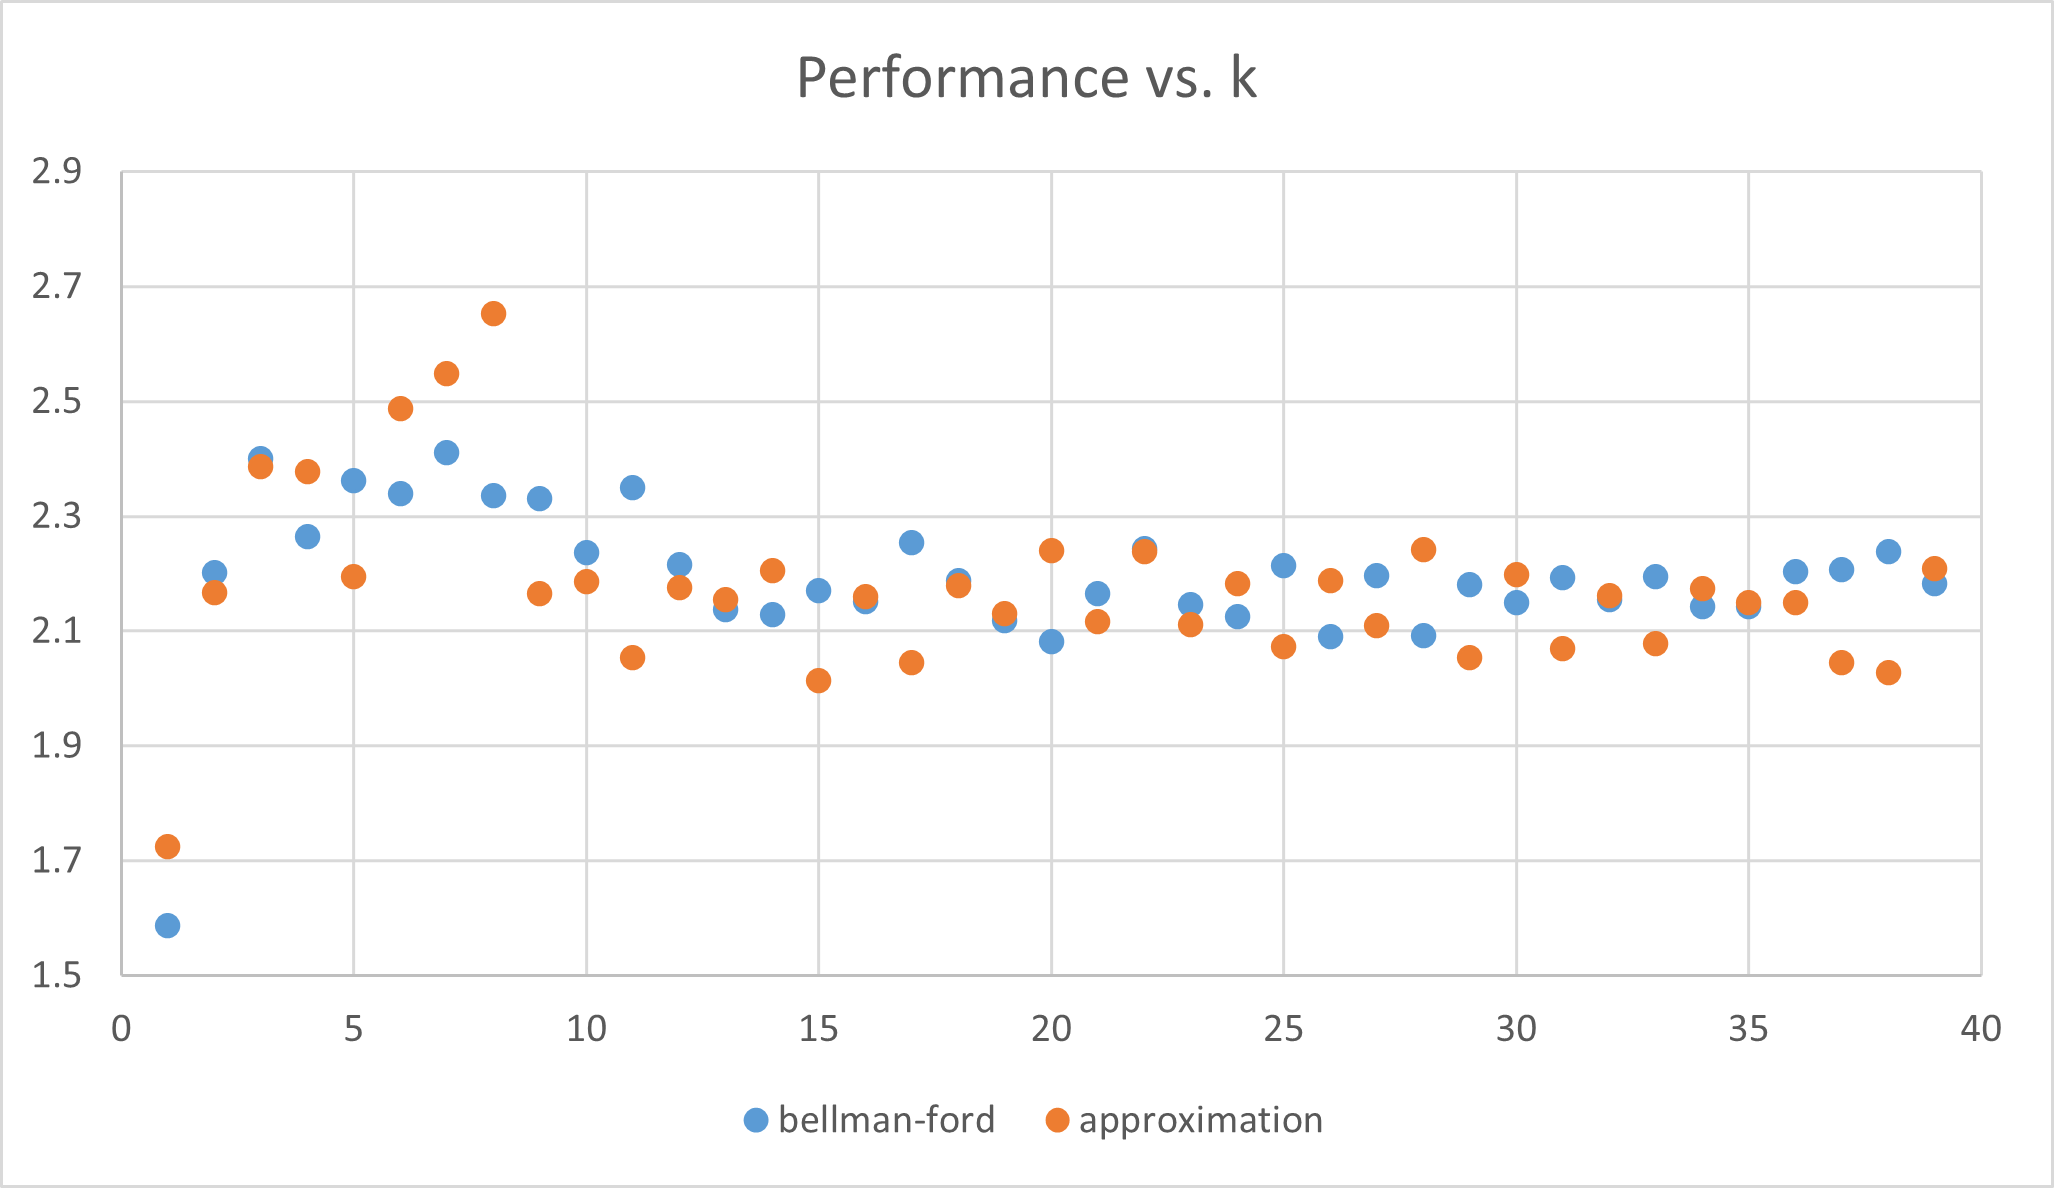
\includegraphics[width=0.7\textwidth,height=\textheight,keepaspectratio]{bellman_ford_time.png}
\caption{performance of bellman-ford and an approximation vs. k}
\label{Figure: m1}
\end{figure}

\subsection{Approximation Testing}

\begin{figure}[H]
\centering
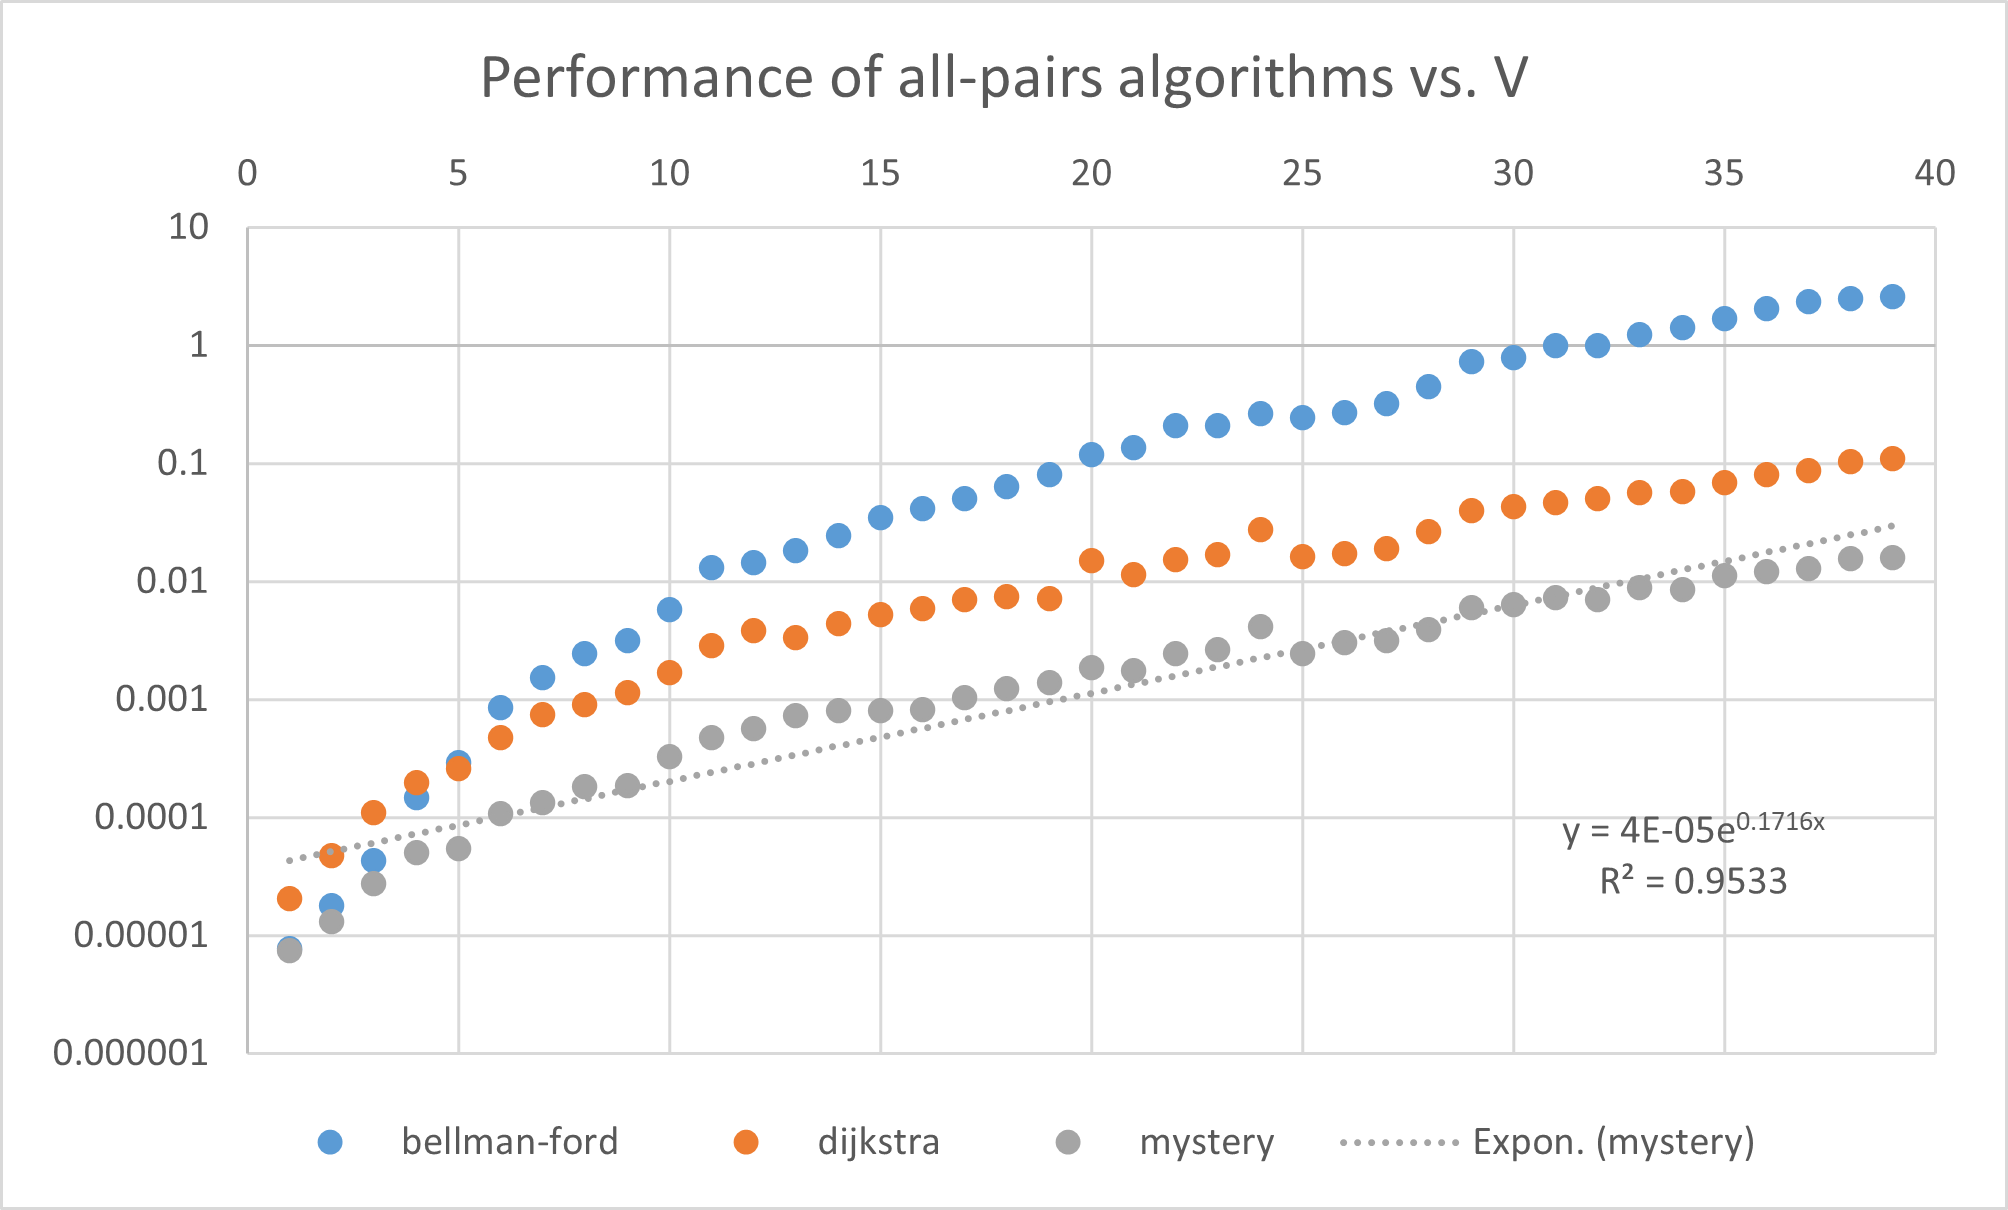
\includegraphics[width=0.7\textwidth,height=\textheight,keepaspectratio]{mystery.png}
\caption{performance of mystery function vs. V}
\label{Figure: m3}
\end{figure}


\end{document}

